\subsubsection{Pod}
	The construction of the tube is driven by the configuration of the pod. Consequently, the system model is constructed such that the pod design configuration is analyzed first. The pod group contains all subsystems onboard the pod. The pod takes in user variables set by the user and feeds them into drag, cycle, drivetrain, geometry, mass, and levitation subsystems. When executed, the pod group outputs all relevant information about the pod configuration and design needed to evaluate system performance \note[Colin]{seems like this could be 1-2 sentence}.
\subsubsection{Tube}
	Once the pod group determines the design configuration of the pod, the tube group is able to analyze the tube design. The tube group contains subsystem analyses for the vacuum pumps, the electromagnetic propulsion system, thermal management, and tube structure. Once the major aspects of the design of the tube are evaluated, results for both pod and tube design can be fed into mission and cost analyses to evaluate overall system performance requirements and their resulting costs\note[Colin]{seems like this could be 1-2 sentence}.
\subsubsection{Mission}
	It is necessary to obtain a reasonable estimation of the mission performance requirements in order to carry out system level trade studies. It is important to note that the exact mission route is dependent on the topography of the land between the two notional endpoints. Currently, it is beyond the scope of the model to account for the effect that varying topology will have on the pod’s trajectory. For simplicity, the model is assumed to travel in a straight, flat line between the departure and arrival locations, in this case the LAX and SFO airports. The mission velocity profile contains three phases: acceleration, coasting with periodic boosting sections, and deceleration\note[Colin]{shorten up text}\note[Colin]{how large do our figures need to be?}.
	\begin{figure}
		\centering
		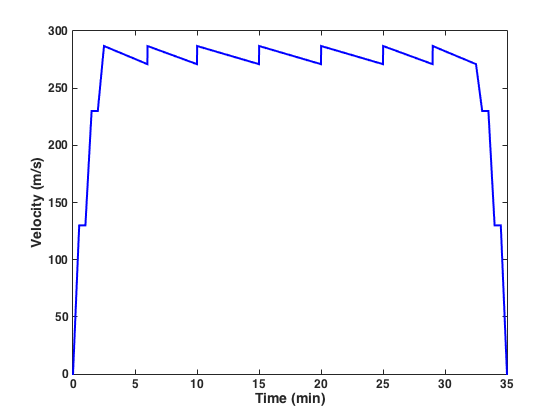
\includegraphics{../images/mission_profile.png}
		\caption{Notional Velocity Profile in Mission Analysis}
		\label{fig:mission_profile}
	\end{figure}
	\Cref{fig:mission_profile} shows what a possible velocity profile would look like using this mission analysis model. The initial acceleration is modeled as a constant linear acceleration of 1g from rest to top speed. Previous analyses have modeled the start up as an incremental acceleration, as is shown in \cref{fig:mission_profile}, due to allow for more maneuverability and to avoid sustaining potentially uncomfortable g forces for to prolonged periods of time \cite{Chin}. This produces a negligible difference in energy consumption from the model used in this analysis. The second phase of travel consists of a coasting pod with periodic boosting sections. In this phase, the pod begins at top speed and is allowed to coast until it reaches some minimum speed set by the user. Then, the will enter an electromagnetic boosting section which will accelerate the pod at 1g back to the desired top speed. For straight and level travel, the acceleration of the pod is given by the equation
	\begin{equation}
		\label{eq:acceleration}
		\frac{\mathrm{d} v}{\mathrm{d} t} = f ( v  ) = \frac{1}{m} ( F_{thrust} - \frac{1}{2}C_{D}\rho V^{2}S - D_{mag})
	\end{equation}
	where $F_{thrust}$ is the net thrust generated by the flow through the pod nozzle, $C_D$ \note[Colin]{let's be sure to consistently use C_D or C_d, minding case} is the pod drag coefficient, $\rho$ is the free stream air density, $S$ is the pod planform area, and $D_{mag}$ is the drag produced by the magnetic levitation system. If the net thrust generated by the nozzle, then the acceleration equation is integrated to find the time and distance it takes for the pod to decelerate to the desired minimum speed using a predictor-corrector integration method \note[Colin]{do we need to include this equation at all?}
	\begin{equation}
		\label{eq:predictor_corrector}
		v_{i+1}^{0} = v_{i}+f(v)\Delta t
	\end{equation}	
	\begin{equation}
		\label{eq:predictor_corrector_2}
		v_{i+1} = v_{i}+\frac{f(v_{i+1}^{0})+f(v_{i})}{2}\Delta t
	\end{equation}	
	\begin{equation}
		\label{eq:predictor_corrector_3}
		x_{i+1} = x_{i}+\frac{v_{i+1}+v_{i}}{2}\Delta t
	\end{equation}	
	The coast distance is used to determine the number of propulsive sections needed along the track to complete the mission. The energy is consumed in a single propulsive section is then multiplied by the number of flights determined from coasting distance to determine the electromagnetic propulsive energy consumed per flight during the coasting phase of the mission. The final phase of the mission is a constant linear deceleration of .5g from top speed to rest. Many systems driven by electromagnetic propulsion conserve energy through regenerative breaking \cite{inductrack}. For the sake of conservatism, it is assumed that there is no regenerative breaking in this process, although the model allows for regenerative breaking to be accounted for if the user desires. The energy consumed per flight is computed by adding the consumption of all three phases. The total yearly energy consumption is calculated based on the frequency of flights, which is determined by the user.

\subsubsection{Cost}
	The cost module estimated the cost of energy, materials, pods, and construction capital. The cost of construction is highly subjective and is difficult to get an accurate estimation within less than an order of magnitude of uncertainty. However, the cost of materials and energy consumption can be estimate with significantly greater certainty. Thus, in this analysis, the cost estimations of materials and energy are of greater interest. According to the Electricity Information Administration, the average price of electricity is about .13 USD/kWh \cite{EIA}. This is the electricity price that will be used for the model. Different electricity prices can be used for future analyses if necessary, but will not change the trends in the data this model produces. In addition to trade studies, a rough estimation of the ticket cost is included, which projects ticket cost based on the equation
	\begin{equation}
		\label{eq:ticket_cost}
		Cost_{ticket} = \frac{ (\frac{\partial Cost}{\partial L}L+\frac{\partial Cost }{\partial pod}n_{pods}+Cost_{capital} ( 1+ib ) + \frac{\partial Cost}{\partial Energy} (Energy_{tube} + Energy_{pod}  ))  )}{n_{passengers}*\frac{pods}{s}*3600\frac{s}{hr}*24\frac{hrs}{day}*365\frac{days}{year}*bm}
	\end{equation}
	Where $ib$ is the bond interest rate, $bm$ is the number of years for bond maturity, and $L$ is the total length of the track. Previous research indicated that construction costs are likely to be the largest cost factor in the system \cite{Musk}. Due to the lack of a reliable method of estimating construction cost or ticket markup at this stage of the design process, the exact values of the ticket cost produced by this model will have a high level of uncertainty. However, the trade studies conducted in these analyses can provide useful information to inform the development of more accurate ticket cost models in the future.